\chapter{Teoremas fundamentales}

\section{Enunciado}
Del circuito de la figura, obtener:
\begin{itemize}
\item Expresiones analíticas de las intensidades $i_1(t)$ e $i_2(t)$
\item Potencia disipada por todas las resistencias
\end{itemize}
Datos: $e_g(t)=50\sqrt{2} \cos(1000\,t)$ V; $i_g(t)=10$ A;
$R_1=R_2=2\Omega$; $R_3=7\Omega$; $L_1=L_2=1$ mH; $L_3=2$ mH

\begin{center}
  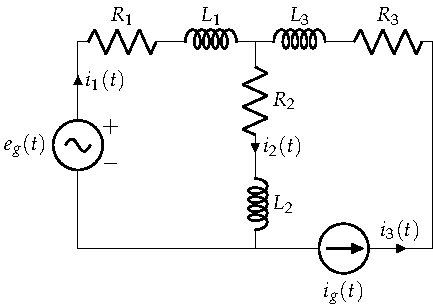
\includegraphics{figuras/BT2_18.pdf}
\end{center}

\subsection*{Solución}

En el circuito hay dos fuentes funcionando a diferentes frecuencias. Por tanto, hay que resolver mediante el principio de superposición.

\textbf{Circuito cuando solo actúa $i_g(t)$}
    
La fuente $e_g(t)$ se cortocircuita y se deja únicamente la fuente
$i_g(t)$. Al ser una fuente de continua, las bobinas se
cortocircuitan. Queda un circuito de dos mallas, donde se sabe que
$I_3'=10$ A. Resolviendo el circuito (por leyes básicas, mallas o
nudos), se obtiene que:
\begin{align*}
  I_1'&=-5\,A\\
  I_2'&=5\,A
\end{align*}
    
Las potencias en este caso:
\begin{align*}
  P_{R1}'&=R_1\,I_1'^2=2\cdot (-5)^2=50\,W\\
  P_{R2}'&=R_2\,I_2'^2=2\cdot 5^2=50\,W\\
  P_{R3}'&=R_3\,I_3'^2=7\cdot 10^2=700\,W\\
\end{align*}
    
\textbf{Circuito cuando solo actúa $e_g(t)$}
    
La fuente $i_g(t)$ queda como un circuito abierto; por tanto, queda un
circuito de una malla e $I_3''=0$ A. Se calculan las reactancias de
las bobinas $L_1$ y $L_2$, sabiendo que $\omega=1000$ rad/s:
\begin{equation*}
  \overline{X_{L1}}=\overline{X_{L2}}=\mathrm{j}\omega L=\mathrm{j}\, 1000\cdot 0.001 = \mathrm{j}\Omega
\end{equation*}
Por la ley de Ohm, tomando valores eficaces, se obtiene el valor de
$\overline{I_1''}=\overline{I_2''}$:
\begin{equation*}
  \overline{I_1''}=\overline{I_2''}=\dfrac{\overline{U}}{\overline{Z_{eq}}}=\dfrac{50\phase{0^\circ}}{2+\mathrm{j}+2+\mathrm{j}}=\underbrace{5\sqrt{5}}_{11.18}\phase{-26.57^\circ} A
\end{equation*}
    
Las potencias en este caso:
\begin{align*}
  P_{R1}''&=R_1\,I_1''^2=2\cdot (5\sqrt{5})^2=250\,W\\
  P_{R2}''&=R_2\,I_2''^2=2\cdot (5\sqrt{5})^2=250\,W\\
  P_{R3}''&=R_3\,I_3''^2=7\cdot 0^2=0\,W\\
\end{align*}
    
\textbf{Expresiones temporales}
    
Por tanto, las expresiones de $i_1(t)$, $i_2(t)$ e $i_3(t)$ son:
\begin{align*}
  i_1(t)&= -5+5\sqrt{10}\cos(1000t-0.46) A \\
  i_2(t)&= 5+5\sqrt{10}\cos(1000t-0.46) A \\
  i_3(t)&= 10 A 
\end{align*}
    
\textbf{Cálculo de $P_T$}
    
La potencia activa total consumida por las resistencias es:
\begin{align*}
  P_T&=R_1\,(I_1'^2+I_1''^2)+R_2\,(I_2'^2+I_2''^2)+R_3\,(I_3'^2+I_3''^2)=\\
     &=2\cdot((-5)^2+(5\sqrt{5})^2)+2\cdot(5^2+(5\sqrt{5})^2)+7\cdot (10^2+0^2)={1300\,W}
\end{align*}
que coincide con el valor obtenido al sumar las potencias de cada
circuito (debido a la ortogonalidad de las señales implicadas):
\begin{equation*}
  P_T=P_{R1}'+P_{R2}'+P_{R3}'+P_{R1}''+P_{R2}''+P_{R3}''=50+50+700+250+250+0=1300\,W
\end{equation*}

%%%%%%%%%%%%%%%%%%%%%%%%%%%%%%%%%%%%%%%%%%%%%%%%%%%%%%%%%%%%%%%%%%

\section{Enunciado}
En el circuito de la figura determina:
\begin{itemize}
\item $u_R(t)$ y $u_L(t)$
\item Balance de potencias
\end{itemize}
Datos:
\begin{equation*}
  e_a(t) = \qty[parse-numbers=false]{3\sqrt{2} \sin(10^3 t)}{\volt}; e_b(t) = \qty[parse-numbers=false]{30\sqrt{2} \sin(10^4 t)}{\volt}; R = \qty{30}{\ohm}; L = \qty{3}{\milli\henry} 
\end{equation*}

\begin{center}
  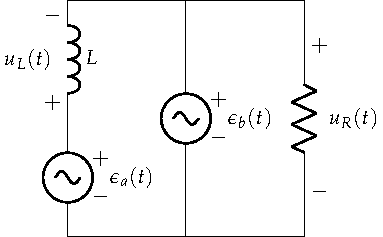
\includegraphics{figuras/superposicion2_ej.pdf}
\end{center}

\subsection*{Solución}

Dado que las fuentes trabajan a frecuencias diferentes, hay que resolver mediante superposición.

Activamos una de las fuentes:
\begin{center}
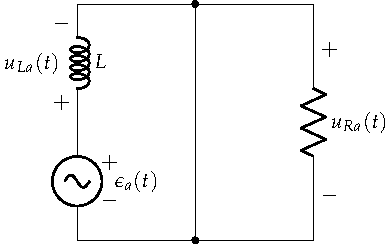
\includegraphics{figuras/superposicion2_A}
\end{center}

La resistencia está cortocircuitada. Por tanto:

\begin{align*}
  u_{Ra}(t) &= \qty{0}{\volt}\\
  u_{La}(t) &= \epsilon_a(t)\\  
\end{align*}

En este circuito la potencia disipada por la resistencia es $P_{Ra} = \qty{0}{\watt}$ y, en consecuencia, la potencia entregada por el generador es $P_{\epsilon_a} = \qty{0}{\watt}$.

Hacemos el análisis con la otra fuente:

\begin{center}
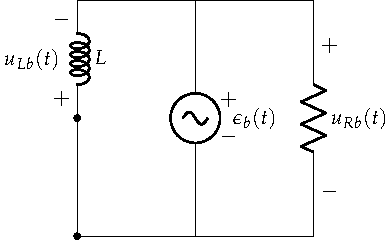
\includegraphics{figuras/superposicion2_B}
\end{center}

En este circuito:

\begin{align*}
  u_{Rb}(t) &= \epsilon_b(t)\\
  u_{Lb}(t) &= -\epsilon_b(t)\\  
\end{align*}

El balance de potencias es:

\begin{equation*}
  P_{Rb} = \frac{\epsilon_b^2}{R_b} = \qty{30}{\watt} = P_{\epsilon_b}\\
\end{equation*}

Por tanto:

\begin{align*}
  u_R(t) &= u_{Ra}(t) + u_{Rb}(t) = 30\sqrt{2}\sin(10^4 t)\\
  u_L(t) &= u_{La}(t) + u_{Lb}(t) = 3\sqrt{2}\sin(10^3 t) - 30\sqrt{2}\sin(10^4 t)\\
\end{align*}

Además, dado que las dos señales de los generadores son ortogonales, podemos sumar las potencias calculadas en cada circuito:

\begin{align*}
  P_R &= P_{Ra} + P_{Rb} = \qty{30}{\watt}\\
  P_\epsilon &= P_{\epsilon_a} + P_{\epsilon_b} = \qty{30}{\watt}\\
\end{align*}

%%%%%%%%%%%%%%%%%%%%%%%%%%%%%%%%%%%%%%%%%%%%%%%%%%%%%%%%%%%%%%%%%%

\section{Enunciado}
El circuito de la figura se encuentra en régimen permanente. Determinar analíticamente la expresión de $i(t)$, así como las potencias entregadas por los generadores y disipadas por las resistencias $R_1$ y $R_2$.

Datos:
\begin{align*}
  e_1(t) = \qty[parse-numbers=false]{50 \sin(1000 t)}{\volt};
  e_2(t) = \qty{30}{\volt};
  R_1 = \qty{6}{\ohm};
  R_2 = \qty{6}{\ohm};
  L = \qty{8}{\milli\henry};
  C = \qty{10}{\micro\farad}
\end{align*}

\begin{center}
  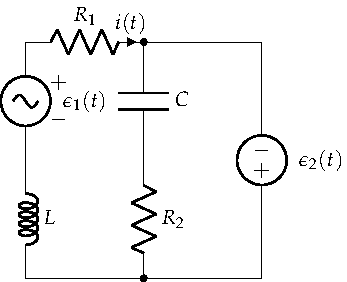
\includegraphics{figuras/superposicion1_ej.pdf}
\end{center}

 \subsection*{Solución}

Aplicamos superposición.

Analizamos con la fuente de corriente alterna:

\begin{center}
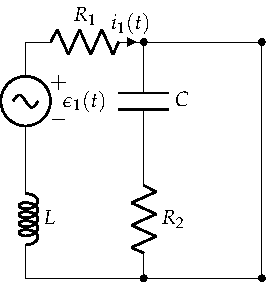
\includegraphics{figuras/superposicion1_AC}
\end{center}

La rama $R_2 - C$ está cortocircuitada y, por tanto, podemos prescindir de ella:

\begin{align*}
  \overline{Z}_1 &= R_1 + jX_L = 6 + 8j\si{\ampere}\\
  \overline{I}_1 &= \overline{\epsilon}_1 / \overline{Z}_1 = 5\sqrt{2}/2\phase{\ang{-53.13}}\si{\ampere}
\end{align*}

En el dominio del tiempo obtenemos:

\begin{equation*}
  i_1(t) = 5\sin(1000t - 0.9273)\si{\ampere}
\end{equation*}

En cuanto al balance de potencias:

\begin{align*}
  P_{R11} &= I_1^2 R_1 = \qty{75}{\watt}\\
  P_{R21} &= \qty{0}{\watt}\\
  P_{\epsilon_1} &= \Re(\overline{\epsilon}_1 \cdot \overline{I}_1^*) = \qty{75}{\watt}
\end{align*}

Analizamos con la fuente de corriente continua:

\begin{center}
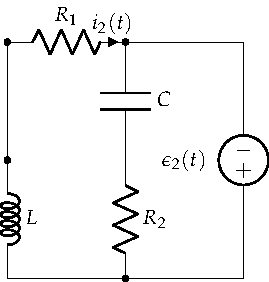
\includegraphics{figuras/superposicion1_DC}
\end{center}

En este circuito sustituimos la bobina por un cortocircuito y el condensador por un circuito abierto. En consecuencia:

\begin{equation*}
  i_2(t) = \epsilon_2(t) / R_1 = \qty{5}{\ampere}
\end{equation*}

En cuanto al balance de potencias:

\begin{align*}
  P_{R12} &= I_2^2 \cdot R_1 = \qty{150}{\watt}\\
  P_{R22} &= \qty{0}{\watt}\\
  P_{\epsilon2} &= \epsilon_2 \cdot I_2 = \qty{150}{\watt}
\end{align*}

Por tanto:

\begin{equation*}
  i(t) = i_1(t) + i_2(t) = 5 + 5\sin(1000t - 0.9273)\si{\ampere}
\end{equation*}

Además, como las señales son ortogonales, podemos hacer el balance de potencias conjunto con los dos circuitos:

\begin{align*}
  P_{R1} &= P_{R11} + P_{R12} = \qty{225}{\watt}\\
  P_{R2} &= P_{R21} + P_{R22} = \qty{0}{\watt}\\
  P_{\epsilon} &= P_{\epsilon1} + P_{\epsilon2} = \qty{225}{\watt}\\
\end{align*}
%%%%%%%%%%%%%%%%%%%%%%%%%%%%%%%%%%%%%%%%%%%%%%%%%%%%%%%%%%%%%%%%%%

\section{Enunciado}
Obtener el generador equivalente de Thévenin del circuito de la figura
respecto de A y B. A partir de este generador, calcula la resistencia
a colocar en AB para obtener la máxima potencia, calculando esta
potencia y la potencia entregada por el generador $\epsilon$.

Datos:
$\epsilon = \qty{54}{\volt};\quad R_1 = R_4 = \qty{8}{\ohm};\quad R_2
= R_3 = \qty{10}{\ohm}$

\begin{center}
  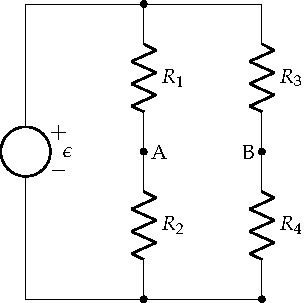
\includegraphics{figuras/Thevenin2}
\end{center}

    
\subsection*{Solución}
Para obtener la tensión $U_{AB}$ aplicamos divisor de tensión en ambas
ramas:

\begin{align*}
  U_A &= \epsilon \cdot \frac{R_2}{R_1 + R_2}\\
  U_B &= \epsilon \cdot \frac{R_4}{R_3 + R_4}\\
  U_{AB} &= \epsilon \cdot (\frac{R_2}{R_1 + R_2} -  \frac{R_4}{R_3 + R_4}) = \qty{6}{\volt} = \epsilon_{th}
\end{align*}

Para calcular la resistencia equivalente apagamos la fuente de
tensión. En el circuito resultante obtenemos:

\begin{equation*}
  R_{th} = (R_1 || R_2) + (R_3 || R_4) = 80/9\si{\ohm}
\end{equation*}

Para obtener la máxima potencia hay que conectar una resistencia
$R_L = R_{th}$. Con esta resistencia el balance de potencias es:

\begin{align*}
  P_L &= \frac{\epsilon_{th}^2}{4R_{th}} = \qty{1.0125}{\watt}\\
  P_\epsilon &= 2 \cdot P_L = \qty{2.025}{\watt}
\end{align*}

%%%%%%%%%%%%%%%%%%%%%%%%%%%%%%%%%%%%%%%%%%%%%%%%%%%%%%%%%%%%%%%%%% 

\section{Enunciado}
Determinar el equivalente Thévenin del circuito de la figura entre los
nudos $A-B$. ¿Qué resistencia habría que conectar en dichos terminales
para transferir la máxima potencia? ¿Cuál sería dicha potencia?

\begin{center}
  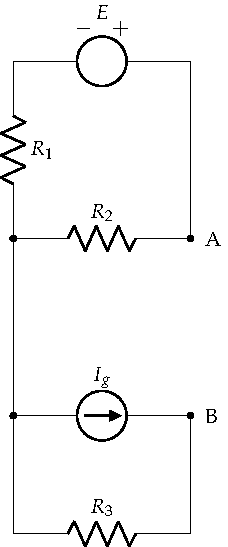
\includegraphics{figuras/BT1_17.pdf}
\end{center}

Datos: $R_1 = R_2 = \qty{4}{\ohm}$; $R_3 = \qty{2}{\ohm}$; $E = \qty{10}{\volt}$; $I_g = \qty{8}{\ampere}$

\subsection*{Solución}
Se transforma la fuente de corriente en paralelo con la resistencia de
$2\Omega$ en una fuente de tensión en serie con dicha resistencia,
como en la figura:
\begin{equation*}
  U_{I_g}=I_g\cdot R_2=8\cdot 2=16\, V
\end{equation*}

\begin{center}
  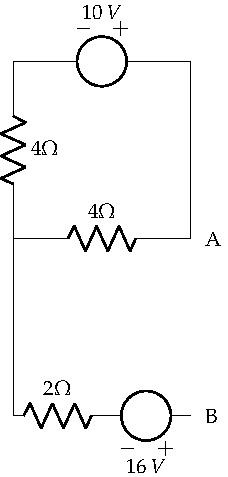
\includegraphics{figuras/BT1_17_mallas.pdf}
\end{center}


\textbf{Cálculo de $\epsilon_{th}$}

Hay que determinar la tensión $U_{AB}$. Considerando el nudo de la
izquierda como masa, y dado que por la resistencia de $2\Omega$ no
circula corriente (circuito abierto entre $A-B$), la tensión en $B$
es:
\begin{equation*}
  U_B=16\,V
\end{equation*}
Aplicando la ley de Ohm a la malla superior:
\begin{equation*}
  I=\dfrac{10}{4+4}=\qty{1.25}{\ampere}
\end{equation*}
por lo que la tensión en el punto $A$:
\begin{equation*}
  U_A=4\cdot 1.25=5\,V
\end{equation*}
Así, la tensión $U_{AB}=\epsilon_{th}$:
\begin{equation*}
  U_{AB}=U_A-U_B=\epsilon_{th}=5-16=-11\,V
\end{equation*}

\textbf{Cálculo de $R_{th}$}

Al no haber fuentes dependientes, se puede obtener esta resistencia
como la $R_{eq}$ vista desde los terminales $A-B$, anulando las
fuentes:
\begin{equation*}
  R_{eq}=R_{th}=2+\dfrac{4\cdot 4}{4+4}=4\Omega
\end{equation*}

\textbf{Equivalente Thévenin} El equivalente de Thévenin queda como se
muestra a continuación:

\begin{center}
  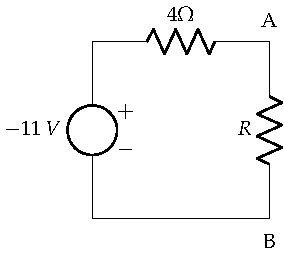
\includegraphics{figuras/BT1_17_th.pdf}
\end{center}

Aplicando el T. Máx. Trans. Potencia, la resistencia a conectar es:
\begin{equation*}
  R_L=R_{th}=4\Omega
\end{equation*}
siendo la máxima potencia transferida:
\begin{equation*}
  P_{max}=\dfrac{\epsilon_{th}^2}{4\,R_{th}}=\dfrac{(-11)^2}{4\cdot 4}=7.56\,W
\end{equation*}

%%%%%%%%%%%%%%%%%%%%%%%%%%%%%%%%%%%%%%%%%%%%%%%%%%%%%%%%%%%%%%%%%%

\section{Enunciado}
Obtener el generador equivalente de Thévenin del circuito de la figura respecto de A y B.

Datos: $I_g=\qty{10}{\ampere}; R_1=\qty{1}{\ohm}; \alpha=5$
\begin{center}
  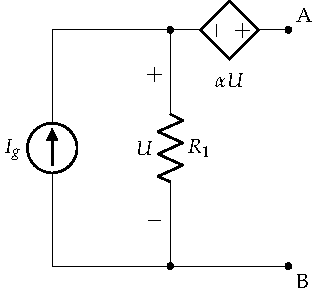
\includegraphics{figuras/Thevenin1.pdf}
\end{center}

\subsection*{Solución}
Por una parte:
\begin{equation*}
  U_{AB} = \alpha U + U = (1 + \alpha) U=(1+5)U=6\,U
\end{equation*}
Además:
\begin{equation*}
  U = I_g \cdot R_1=10\cdot 1 = 10\,V
\end{equation*}
Por tanto, el generador de Thévenin tiene una fem de:
\begin{equation*}
  U_{AB} = 6\, U= 6\cdot 10=60 V = \epsilon_{th}
\end{equation*}

Para calcular la impedancia, se apaga la fuente independiente. Como la
fuente dependiente permanece, es necesario aplicar un generador de
prueba a la salida:

\begin{center}
  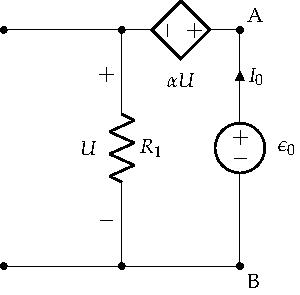
\includegraphics{figuras/Thevenin1_fuenteprueba.pdf}
\end{center}

\begin{align*}
  \epsilon_0 &= \alpha U + U = U(1+\alpha)=6\,U\\
  U &= I_0\,R_1=I_0\cdot 1=I_0
\end{align*}
Por tanto,

\begin{equation*}
  R_{th} = \dfrac{\epsilon_0}{I_0}=\dfrac{6\,U}{U} = 6 \Omega
\end{equation*}

%%%%%%%%%%%%%%%%%%%%%%%%%%%%%%%%%%%%%%%%%%%%%%%%%%%%%%%%%%%%%%%%%%

\section{Enunciado}

En el circuito de la figura, calcular:
\begin{itemize}
\item La corriente del generador equivalente de Norton respecto de A y
  B, $I_N$.
\item La resistencia del generador equivalente de Norton respecto de A
  y B, $R_N$.
\item La resistencia de carga que se debe conectar entre A y B para
  conseguir la máxima potencia disponible, y el valor de esta
  potencia.
\end{itemize}

Datos: $R = {1}{\Omega};\; \epsilon_g = {10}{V};\; \alpha = \qty{1}{\ohm}; \beta = 1$

\begin{center}
  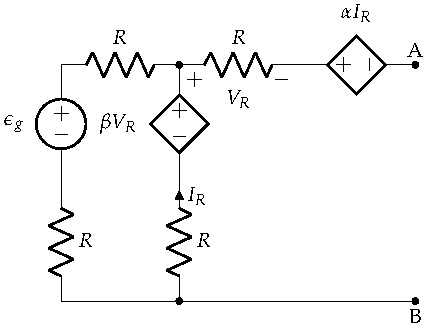
\includegraphics{figuras/norton.pdf}
\end{center}

\subsection*{Solución}
Para calcular el equivalente de Norton cortocircuitamos la salida del circuito. Podemos escribir las siguientes ecuaciones:

\begin{minipage}{0.5\linewidth}
  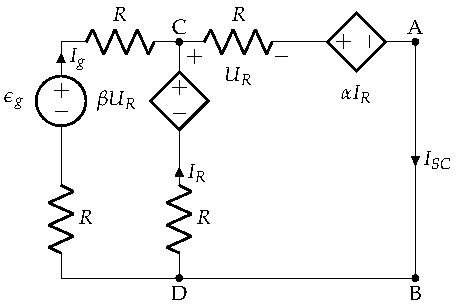
\includegraphics[width=.9\linewidth]{figuras/norton_corto.pdf}
\end{minipage}
\begin{minipage}{0.5\linewidth}
  \begin{align*}
    U_R &= R \cdot I_{sc}\\
    I_g+ I_R &= I_{sc}\\
    U_{CD} &= \epsilon_g - 2 \cdot R \cdot I_g\\
    U_{CD} &= \beta \cdot U_r - I_R \cdot R\\
    U_{CD} &= U_R + \alpha \cdot I_R
  \end{align*}
\end{minipage}

Combinando estas ecuaciones obtenemos:

\begin{equation*}
  I_{sc} = 10/3\si{\ampere} = I_N
\end{equation*}

Para obtener la resistencia equivalente apagamos la fuente independiente y conectamos un generador de prueba en AB:


\begin{minipage}{0.5\linewidth}
  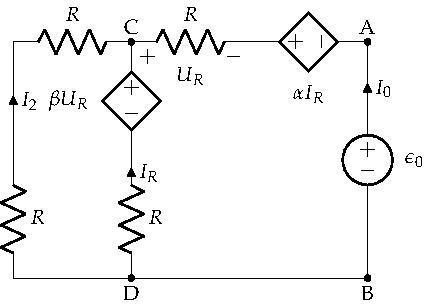
\includegraphics[width=.9\linewidth]{figuras/norton_fuenteprueba.pdf}
\end{minipage}
\begin{minipage}{0.5\linewidth}
  \begin{align*}
    U_R &= -I_0 \cdot R\\
    I_2 + I_R + I_0 &= 0\\
    U_{CD} &= -2R\cdot I_2\\
    U_{CD} &= \beta \cdot U_R - I_R \cdot R\\
    U_{CD} &= U_R + \alpha \cdot I_R + \epsilon_0
  \end{align*}
\end{minipage}

Combinando estas ecuaciones obtenemos:

\begin{equation*}
  R_{th} = \frac{\epsilon_0}{I_0} = \qty{2}{\ohm}
\end{equation*}

Por tanto, habrá que conectar una resistencia de $\qty{2}{\ohm}$ para obtener la máxima potencia disponible.

\section{Enunciado}
Obtén el generador equivalente de Thévenin del circuito de la figura respecto de A y B.

\begin{center}
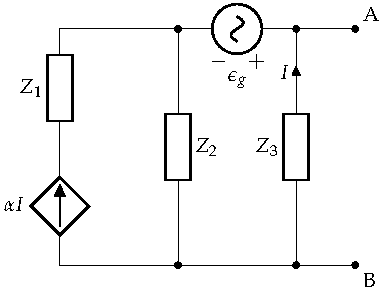
\includegraphics{figuras/Thevenin4}
\end{center}

Datos:
\begin{equation*}
  \overline{\epsilon_g} = \qty[parse-numbers=false]{12 - 16j}{\volt};
  \overline{Z}_1 = \qty[parse-numbers=false]{1 - j}{\ohm};
  \overline{Z}_2 = \qty[parse-numbers=false]{1 + j}{\ohm};
  \overline{Z}_3 = \qty[parse-numbers=false]{5 + 3j}{\ohm}
  \alpha = 2
\end{equation*}


\subsection*{Solución}

Dejamos el circuito en abierto y calculamos la tensión en AB:

\begin{align*}
  \overline{U}_{AB} &= \overline{\epsilon}_g + (1 + \alpha) \overline{I} \cdot \overline{Z}_2\\
  \overline{U}_{AB} &= - \overline{I} \cdot \overline{Z}_3
\end{align*}

Combinando estas ecuaciones obtenemos la tensión:

\begin{equation*}
  \overline{\epsilon}_{th} = \overline{U}_{AB} = \frac{\overline{\epsilon}_g}{1 + (1 + \alpha) \frac{\overline{Z}_2}{\overline{Z}_3}} = 6 - 10j = 11.66\phase{\ang{-59.04}}\si{\volt}
\end{equation*}

Para obtener la impedancia apagamos las fuentes independientes. Como hay fuentes dependientes debemos aplicar una fuente de prueba a la salida del circuito, con fuerza electromotriz $\overline{\epsilon}_0$ y corriente inyectada $\overline{I}_0$.

\begin{minipage}{0.5\linewidth}
  \begin{center}
    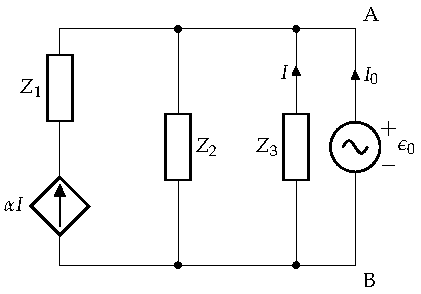
\includegraphics{figuras/Thevenin4_fuenteprueba}
  \end{center}
\end{minipage}
\begin{minipage}{0.5\linewidth}
  \begin{align*}
    \overline{\epsilon}_0 &= [(1 + \alpha) \overline{I} + \overline{I}_0] \cdot \overline{Z}_2\\
    \overline{\epsilon}_0 &= - \overline{I}\cdot \overline{Z}_3
  \end{align*}
\end{minipage}

Combinando ambas expresiones obtenemos:

\begin{equation*}
  \overline{Z}_{th} = \frac{\overline{\epsilon}_0}{\overline{I}_0} = \frac{\overline{Z}_2 \cdot \overline{Z}_3}{(1 + \alpha) \overline{Z}_2 + \overline{Z}_3} = 0.64 + 0.52j\si{\ohm}
\end{equation*}

Para obtener la máxima potencia disponible hay que conectar una impedancia:
\begin{equation*}
\overline{Z}_L = \overline{Z}^*_{th} = 0.64-0.52j\si{\ohm}
\end{equation*}

Esta impedancia disipará una potencia:
\begin{equation*}
P_L = \frac{\epsilon_{th}^2}{4 \cdot R_{th}} = \qty{53.11}{\watt}
\end{equation*}

%%%%%%%%%%%%%%%%%%%%%%%%%%%%%%%%%%%%%%%%%%%%%%%%%%%%%%%%%%%%%%%%%%

\section{Enunciado}

Obtén el generador equivalente de Thévenin del circuito de la figura respecto de A y B. A partir de este generador, calcula la impedancia a colocar en AB para obtener la máxima potencia, calculando esta potencia.

\begin{minipage}{0.5\textwidth}
\begin{center}
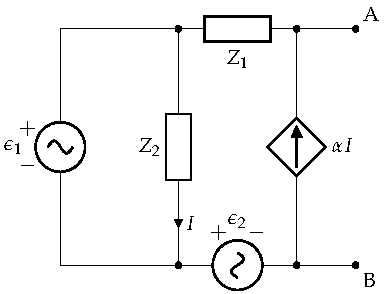
\includegraphics{figuras/Thevenin5}
\end{center}
\end{minipage}
\begin{minipage}{0.5\textwidth}
  \begin{align*}
    \overline{\epsilon_1} &= \SI[parse-numbers=false]{10\phase{0}}{\volt}\\
    \overline{\epsilon_2} &= \SI[parse-numbers=false]{10j}{\volt}\\
    \overline{Z}_1 &= \SI[parse-numbers=false]{4 - 3j}{\ohm}\\
    \overline{Z}_2 &= \SI[parse-numbers=false]{3 + 4j}{\ohm}\\
    \alpha &= 2
  \end{align*}
\end{minipage}
\subsection*{Solución}

La tensión en circuito abierto es:

\begin{equation*}
  \overline{U}_{AB} = \alpha \overline{I} \cdot \overline{Z}_1 + \overline{\epsilon}_1 + \overline{\epsilon}_2
\end{equation*}
siendo $\epsilon_1 = \overline{Z}_2 \cdot \overline{I}$. Por tanto,

\begin{equation*}
  \epsilon_{th}  = \alpha \cdot \overline{\epsilon}_1 \cdot \frac{\overline{Z}_1}{\overline{Z}_2} + \overline{\epsilon}_1 + \overline{\epsilon}_2 = 10 - 10j \si{\volt}
\end{equation*}

Para obtener la impedancia apagamos las fuentes independientes. Al apagar la fuente $\epsilon_1$, la impedancia $Z_2$ queda cortocircuitada y, por tanto, $I = 0$. En consecuencia, la fuente dependiente también queda apagada y obtenemos:

\begin{equation*}
  \overline{Z}_{th} = \overline{Z}_1 = 4 - 3j \si{\ohm}
\end{equation*}

Para obtener la máxima potencia debemos conectar la impedancia:

\begin{equation*}
  \overline{Z}_{L} = \overline{Z}^*_{th} = 4 + 3j \si{\ohm}
\end{equation*}

El balance de potencias es:

\begin{align*}
  P_L &= \frac{\epsilon_{th}^2}{4 \cdot R_{th}} = \SI{12.5}{\watt}\\
  P_{\epsilon} &= 2 \cdot P_L = \SI{25}{\watt} 
\end{align*}

%%%%%%%%%%%%%%%%%%%%%%%%%%%%%%%%%%%%%%%%%%%%%%%%%%%%%%%%%%%%%%%%%%

%%% Local Variables:
%%% mode: latex
%%% TeX-master: "Problemas_TC"
%%% ispell-local-dictionary: "castellano"
%%% End:
